\documentclass[11pt,letterpaper]{article}
\usepackage[utf8]{inputenc}
\usepackage[T1]{fontenc}
\usepackage[spanish,es-tabla]{babel}
\usepackage{lmodern}
\usepackage[margin=2.5cm]{geometry}
\usepackage{amsmath,amssymb,amsthm,bm}
\usepackage{booktabs,array,multirow}
\usepackage{graphicx}
\usepackage{float}
\usepackage{xcolor}
\usepackage{enumitem}
\usepackage{tikz}
\usetikzlibrary{backgrounds,fit,positioning}
\usepackage{quantikz}
\usepackage[colorlinks=true,linkcolor=blue!50!black,citecolor=blue!50!black,urlcolor=blue!50!black]{hyperref}
\usepackage{caption}
\captionsetup{font=small,labelfont=bf}

\providecommand{\ket}[1]{\left|#1\right\rangle}
\providecommand{\bra}[1]{\left\langle#1\right|}
\providecommand{\braket}[2]{\left\langle#1\middle|#2\right\rangle}
\newcommand{\R}{\mathbb{R}}
\DeclareMathOperator{\softmax}{softmax}
\DeclareMathOperator*{\argmax}{arg\,max}

\title{\textbf{Metodología del proyecto:}\\[2pt]
Clasificación de variedades de frijol seco con una red neuronal cuántica de \emph{data re-uploading}}
\author{Computación Cuántica -- Proyecto Final (Opción 1: Clasificación de Semillas)\\
Prof.\ Naomi Itzel Reyes Granados \;\;|\;\; Ayud.\ Sebastián González Juárez}
\date{Entrega: 7 de diciembre de 2026}

\begin{document}
\maketitle

\begin{abstract}
\noindent Este documento describe de forma detallada y justificada la metodología seguida en el
proyecto: el planteamiento del problema, el tratamiento de los datos (incluyendo las medidas contra
la fuga de información), el fundamento teórico del clasificador cuántico variacional elegido
(\emph{data re-uploading}), su implementación híbrida cuántico-clásica, el diseño experimental y la
forma de evaluar y comparar contra modelos clásicos. Se incluyen las decisiones de diseño y su
justificación, así como las limitaciones. Todo el código y los resultados reproducibles se
encuentran en el cuaderno \texttt{Proyecto\_Final\_Semillas\_QML.ipynb}.
\end{abstract}

\tableofcontents
\bigskip

%=====================================================================
\section{Planteamiento del problema}
%=====================================================================
\subsection{Contexto (narrativa)}
Una cooperativa agrícola y centro de acopio de leguminosas recibe a diario toneladas de frijol de
distintos productores. El precio, las condiciones de almacenamiento y la certificación de semilla
dependen de la \emph{variedad}, y mezclar variedades (impureza varietal) puede inutilizar un lote
completo. La clasificación manual por personal experto es lenta, subjetiva y cansada.

El centro cuenta con una banda transportadora con cámara que, mediante visión por computadora,
extrae para cada grano 16 medidas morfológicas (área, perímetro, longitudes de los ejes, factores de
forma, etc.). El problema consiste en \textbf{decidir, a partir de esas medidas, a cuál de siete
variedades pertenece cada grano}: Barbunya, Bombay, Cali, Dermason, Horoz, Seker y Sira.

\subsection{Pregunta de investigación y objetivos}
\begin{quote}
\emph{¿Puede un clasificador variacional cuántico de muy pocos qubits y parámetros competir con
modelos clásicos de tamaño comparable en este problema multiclase real, y qué se gana o se pierde
al hacerlo?}
\end{quote}
Objetivos específicos: (i) formalizar el problema; (ii) diseñar un preprocesamiento sin fuga de
información y compatible con la codificación cuántica; (iii) implementar y entrenar una QNN de
\emph{data re-uploading}; (iv) compararla con baselines clásicos usando métricas adecuadas
(\emph{accuracy}, F1 macro, matriz de confusión); (v) analizar la influencia de la arquitectura
(ablaciones) y del muestreo finito (\emph{shots}), y discutir con honestidad la existencia o no de
ventaja cuántica.

\subsection{Formalización}
Sea $\mathcal{D}=\{(\bm{x}_i,y_i)\}_{i=1}^{N}$, con $\bm{x}_i\in\R^{16}$ y
$y_i\in\{0,\dots,6\}$. Se busca un clasificador probabilístico
$f_{\bm\theta}:\R^{d}\to\Delta^{6}$ (símplex de probabilidades sobre las 7 clases) que minimice la
entropía cruzada empírica
\begin{equation}
\mathcal{L}(\bm\theta)= -\frac{1}{N}\sum_{i=1}^{N}\log\big[f_{\bm\theta}(\bm{x}_i)\big]_{y_i},
\qquad
\hat{y}(\bm{x})=\argmax_{k}\,[f_{\bm\theta}(\bm{x})]_k .
\label{eq:loss}
\end{equation}
La entropía cruzada es la log-verosimilitud negativa de un modelo categórico; es diferenciable, y
su minimización con modelos suficientemente expresivos aproxima las probabilidades condicionales
$P(y\mid\bm{x})$. Dado que $\bm\theta$ incluye ángulos de rotaciones, el problema de optimización
es \textbf{no convexo}, por lo que el resultado depende de la inicialización y se mide con varias
semillas.

%=====================================================================
\section{Datos}
%=====================================================================
Se usa el conjunto \emph{Dry Bean} del repositorio UCI \cite{koklu2020}: 13\,611 granos de siete
variedades, fotografiados y segmentados, con 16 características: 12 dimensiones/geometrías (área,
perímetro, longitud del eje mayor y menor, razón de aspecto, excentricidad, área convexa, diámetro
equivalente, \emph{extent}, \emph{solidity}, \emph{roundness}, \emph{compactness}) y 4 factores de
forma.

\paragraph{Calidad de datos.} No hay valores nulos. Se detectaron \textbf{68 filas duplicadas
exactas} que se eliminaron (quedan 13\,543 granos): un grano repetido que cayera en entrenamiento y
prueba a la vez inflaría artificialmente el desempeño (fuga de información).

\paragraph{Desbalance.} La clase mayoritaria (Dermason, $\approx 26\%$) es unas siete veces más
frecuente que la minoritaria (Bombay, $\approx 4\%$). Por ello se usa partición \emph{estratificada}
y se reporta F1 macro además de \emph{accuracy}.

\paragraph{Redundancia.} Hay 15 pares de características con $|\rho|>0.95$ (área, perímetro, ejes,
diámetro equivalente, área convexa\ldots). Esto motiva la reducción de dimensionalidad.

\begin{figure}[H]
\centering
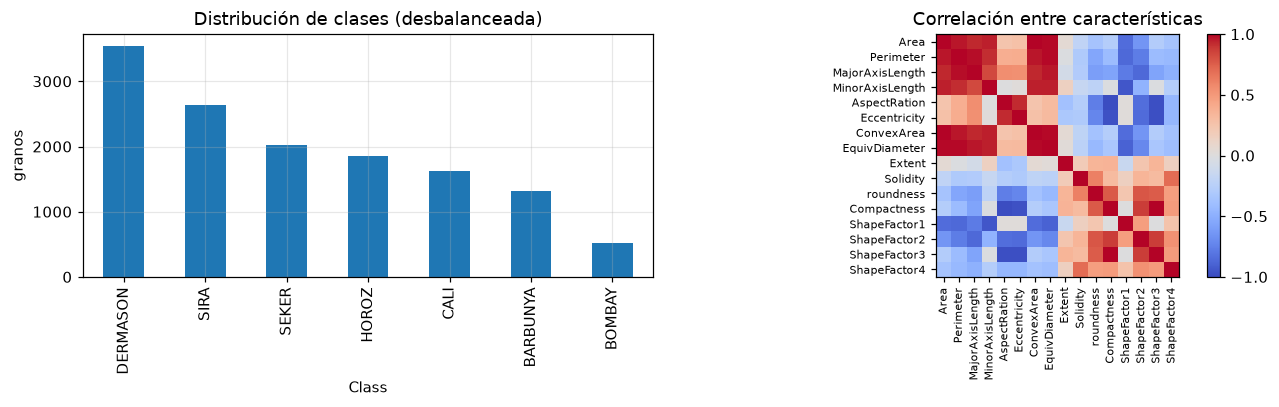
\includegraphics[width=\textwidth]{figures/eda.png}
\caption{Izquierda: distribución de clases. Derecha: matriz de correlación; los bloques rojos
indican fuerte redundancia entre características.}
\end{figure}

%=====================================================================
\section{Preprocesamiento sin fuga de información}
%=====================================================================
La codificación cuántica impone dos restricciones: (a) con \emph{codificación por ángulos} se usa un
qubit por característica, y el costo de simular o ejecutar el circuito crece rápidamente con el
número de qubits; (b) los datos deben transformarse a ángulos en un intervalo acotado. El pipeline
es el siguiente y \textbf{todos sus parámetros se ajustan únicamente con el conjunto de
entrenamiento}:

\begin{enumerate}[leftmargin=*]
\item \textbf{Partición estratificada.} 70\,\% entrenamiento / 30\,\% prueba (4\,063 granos); del
entrenamiento se aparta 10\,\% como \emph{validación} (948 granos) para elegir la mejor época. El
conjunto de prueba se usa una sola vez al final. Resultan 8\,532 / 948 / 4\,063 granos.
\item \textbf{Estandarización} (media 0, varianza 1). Es indispensable antes de PCA, pues las
características tienen escalas muy diferentes (área $\sim10^{5}$ frente a razones $\sim1$).
\item \textbf{PCA a 4 componentes} (uno por qubit), que retiene aprox.\ $95\%$ de la varianza
(Figura~\ref{fig:pca}). Se ajusta con train y se aplica a validación y prueba.
\item \textbf{Escalado a $[0,\pi]$} con min--max (ajustado en train). Como $R_X(\alpha x)$ es
$2\pi$-periódica en el ángulo, el rango $[0,\pi]$ mantiene una correspondencia inyectiva entre
valores y estados en la esfera de Bloch (con $[0,2\pi]$ los extremos coincidirían). En validación y
prueba algunos valores pueden salir ligeramente del rango, lo que es esperable.
\end{enumerate}

\begin{figure}[H]
\centering
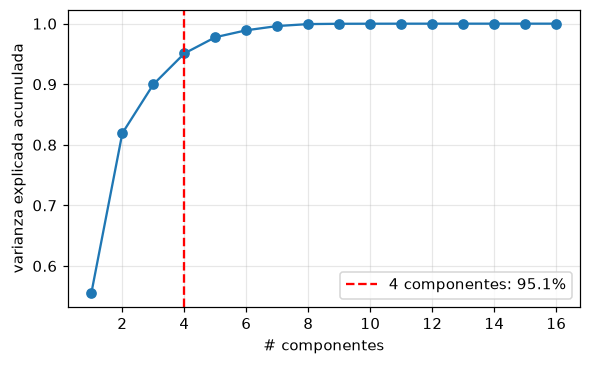
\includegraphics[width=.55\textwidth]{figures/pca.png}
\caption{Varianza explicada acumulada (PCA ajustado en train). Con 4 componentes se conserva
$\approx95\%$.}
\label{fig:pca}
\end{figure}

\paragraph{Justificación de la compresión.} Reducir de 16 a 4 características \emph{pierde} algo de
información discriminante; este costo se cuantifica explícitamente al comparar con modelos
clásicos que sí usan las 16 características (Sección~\ref{sec:res}).

%=====================================================================
\section{Fundamento teórico del modelo cuántico}
%=====================================================================
\subsection{Clasificadores variacionales y el límite de codificar una sola vez}
Un modelo cuántico variacional evalúa $f(\bm{x})=\bra{0}U^\dagger(\bm{x},\bm\theta)\,M\,U(\bm{x},\bm\theta)\ket{0}$
con un circuito $U$ parametrizado y una medición $M$. Schuld, Sweke y Meyer \cite{schuld2021} probaron
que, si el dato se codifica con puertas de la forma $e^{-ix H/2}$, el modelo es una \textbf{serie de
Fourier truncada} en $\bm{x}$:
\begin{equation}
f_{\bm\theta}(x)=\sum_{\omega\in\Omega} c_\omega(\bm\theta)\,e^{i\omega x},
\end{equation}
donde el espectro $\Omega$ queda determinado únicamente por la codificación (los valores propios del
generador), mientras que los coeficientes $c_\omega$ son los que se entrenan. Con una sola subida de
$R_X(x)$ por qubit solo hay frecuencias $\omega\in\{-1,0,1\}$: el modelo es poco expresivo. Si se
codifica $L$ veces, $\Omega=\{-L,\dots,L\}$.

\subsection{Arquitectura \emph{data re-uploading}}
La idea de Pérez-Salinas et al.\ \cite{perez2020} es intercalar $L$ veces \emph{codificación} y
\emph{bloques entrenables}:
\begin{equation}
U_{\bm\theta}(\bm{x})=\prod_{l=L}^{1}\Big[\,W_l(\bm\theta_l)\,S_l(\bm{x};\bm\alpha_l)\Big],\qquad
\ket{\psi(\bm{x})}=U_{\bm\theta}(\bm{x})\ket{0}^{\otimes n},
\end{equation}
\begin{align}
S_l(\bm{x};\bm\alpha_l)&=\bigotimes_{q=1}^{n}R_X(\alpha_{l,q}\,x_q),\\
W_l(\bm\theta_l)&=\underbrace{\mathrm{CNOT}_{n\to1}\cdots\mathrm{CNOT}_{2\to3}\,\mathrm{CNOT}_{1\to2}}_{\text{anillo de entrelazamiento}}
\;\bigotimes_{q=1}^{n}\mathrm{Rot}(\phi_{l,q},\vartheta_{l,q},\omega_{l,q}),
\end{align}
con $\mathrm{Rot}(\phi,\vartheta,\omega)=R_Z(\omega)R_Y(\vartheta)R_Z(\phi)$, una rotación genérica en
SU(2). Los $\alpha_{l,q}$ son \textbf{pesos de escala entrenables}, el análogo de $w\cdot x$ en una
neurona: reescalan los datos y, con ello, los anchos de banda del modelo de Fourier.

\begin{figure}[H]
\centering
\begin{quantikz}[row sep=0.25cm, column sep=0.35cm]
\lstick{$\ket{0}$} & \gate[4,style={fill=blue!10}]{\text{dato}}\gategroup[4,steps=6,style={dashed,rounded corners,inner xsep=2pt},background,label style={label position=above,anchor=south,yshift=-0.1cm}]{\small repetir $L$ veces} & \gate{\mathrm{Rot}} & \ctrl{1} & \qw & \qw & \targ{} & \qw & \meter{} \\
\lstick{$\ket{0}$} & & \gate{\mathrm{Rot}} & \targ{} & \ctrl{1} & \qw & \qw & \qw & \meter{} \\
\lstick{$\ket{0}$} & & \gate{\mathrm{Rot}} & \qw & \targ{} & \ctrl{1} & \qw & \qw & \meter{} \\
\lstick{$\ket{0}$} & & \gate{\mathrm{Rot}} & \qw & \qw & \targ{} & \ctrl{-3} & \qw & \meter{}
\end{quantikz}
\caption{Una capa del circuito ($n=4$). El bloque ``dato'' aplica $R_X(\alpha_{l,q}x_q)$ en cada qubit
$q$; después, una rotación $\mathrm{Rot}$ entrenable por qubit y CNOTs en anillo. Esta capa se repite
$L$ veces (modelo principal: $L=4$) y al final se miden las probabilidades de los estados base.}
\label{fig:circ}
\end{figure}

\subsection{¿Por qué resuelve el problema? (argumento de expresividad)}
\begin{enumerate}[leftmargin=*]
\item \textbf{Frecuencias.} Cada re-subida amplía el espectro de frecuencias accesible
(hasta $\pm L$ por característica), de modo que el modelo puede representar fronteras de decisión
cada vez más complejas (Sección anterior).
\item \textbf{Mezcla de características.} Los CNOT crean entrelazamiento, de manera que las
amplitudes finales dependen de \emph{productos} de funciones trigonométricas de distintas
características, no solo de sumas; es el análogo de las capas ocultas.
\item \textbf{Universalidad.} Pérez-Salinas et al.\ \cite{perez2020} y Schuld et
al.\ \cite{schuld2021} demuestran que, con suficientes capas, esta familia puede aproximar
cualquier función continua acotada (aproximador universal), igual que un MLP con capa oculta ancha.
\item \textbf{Geometría.} Cada capa ``dobla'' el espacio de entrada sobre una trayectoria en el
espacio de Hilbert; la clasificación consiste en que las trayectorias de muestras de la misma clase
terminen cerca del mismo estado base.
\end{enumerate}
La universalidad garantiza \emph{existencia}, no \emph{capacidad de aprenderlo} con un optimizador
local en un paisaje no convexo; por eso la evidencia empírica (ablaciones, Sección~\ref{sec:abl})
es parte esencial de la justificación.

\subsection{Lectura multiclase y función de pérdida}
Con $n=4$ qubits hay $2^4=16$ estados base. Se asocia la clase $k$ al estado $\ket{k}$
($k=0,\dots,6$), y se definen
\begin{equation}
p_k(\bm{x})=\big|\braket{k}{\psi(\bm{x})}\big|^{2},\qquad
f_{\bm\theta}(\bm{x})_k=\softmax_k\big(\beta\,p_k(\bm{x})\big)
=\frac{e^{\beta p_k}}{\sum_{j=0}^{6}e^{\beta p_j}} .
\end{equation}
La temperatura $\beta>0$ es \emph{entrenable}: como $p_k\in[0,1]$, sin ella el \emph{softmax} sería casi
uniforme y la entropía cruzada \eqref{eq:loss} no podría hacerse pequeña. Los 9 estados base
restantes actúan como ``desagüe'' de probabilidad. El número total de parámetros es
\begin{equation}
|\bm\theta|=\underbrace{3nL}_{\mathrm{Rot}}+\underbrace{nL}_{\alpha}+\underbrace{1}_{\beta}=4nL+1
\;\;\Rightarrow\;\; 65\ \text{para } n=4,\ L=4 .
\end{equation}

\subsection{Optimización}
Se minimiza la entropía cruzada por descenso estocástico con \textbf{Adam} (tasa inicial
$0.05$, decaimiento coseno, \emph{minibatch} de 128, 20 épocas). Los ángulos se inicializan
uniformemente en $[0,2\pi)$, $\alpha_{l,q}=1$ y $\beta=10$. Los gradientes se obtienen por
\emph{backpropagation} sobre el simulador de vector de estado, eficiente en simulación. En un
dispositivo real se usaría la regla de desplazamiento de parámetros (\emph{parameter-shift}),
$\partial_\theta f=\tfrac12[f(\theta+\pi/2)-f(\theta-\pi/2)]$, que cuesta dos evaluaciones del circuito
por parámetro y por muestra (Sección~\ref{sec:costo}).

%=====================================================================
\section{Implementación}
%=====================================================================
\subsection{Pila de software y justificación}
\begin{table}[H]
\centering
\small
\begin{tabular}{@{}p{3.1cm}p{11.4cm}@{}}
\toprule
Librería & Uso y justificación \\ \midrule
\texttt{numpy}, \texttt{pandas}, \texttt{matplotlib} & Manejo de datos y gráficas (estándar). \\
\texttt{scikit-learn} & Partición estratificada, estandarización, PCA, métricas y modelos
clásicos de referencia; evita reimplementar piezas bien probadas y garantiza una comparación justa. \\
\texttt{pennylane} & Definición del circuito y diferenciación automática. Su \emph{parameter
broadcasting} evalúa todo un \emph{minibatch} en una sola ejecución del circuito, lo que reduce el
entrenamiento de horas a minutos. \\
\texttt{qiskit} & Verificación cruzada independiente (vector de estado) y transpilación a
compuertas nativas para estimar profundidad en hardware. \\
\bottomrule
\end{tabular}
\end{table}
Se trabajó en un entorno \texttt{conda} dedicado (\texttt{compu\_cuantica}, Python 3.11,
PennyLane 0.45, Qiskit 2.6, scikit-learn 1.9).

\subsection{Verificación del circuito}
El circuito se reconstruyó en Qiskit y se comparó con PennyLane para $L\in\{1,3,4\}$ con
parámetros aleatorios y 20 muestras: la diferencia máxima entre probabilidades fue
$\lesssim5\times10^{-16}$, es decir, precisión de máquina. Transpilado a $\{R_z,\sqrt{X},X,\mathrm{CNOT}\}$,
el modelo $L=4$ tiene \textbf{96 compuertas} (16 CNOT) y \textbf{profundidad 36}.

\subsection{Decisiones de diseño relevantes}
\begin{itemize}[leftmargin=*]
\item \textbf{4 qubits.} Equilibrio entre información (95\,\% de varianza) y costo de simulación.
\item \textbf{Lectura por probabilidades de estados base} con temperatura entrenable: permite
obtener las 7 salidas con una única medición en la base computacional, sin observables ni circuitos adicionales.
\item \textbf{Escala entrenable $\alpha$:} imita la parte lineal de una neurona y facilita adaptar el
ancho de banda a cada característica.
\item \textbf{Selección de época por F1 macro en validación}, nunca en prueba.
\item \textbf{Tres semillas} de inicialización para medir la variabilidad inherente al paisaje no
convexo.
\end{itemize}

%=====================================================================
\section{Diseño experimental y métricas}
%=====================================================================
\paragraph{Métricas.} \emph{Accuracy}; F1 macro (promedio no ponderado del F1 por clase; es la
métrica principal por el desbalance), F1 ponderado; matriz de confusión y reporte por clase
(precisión y exhaustividad).

\paragraph{Baselines clásicos} (mismas particiones; hiperparámetros por defecto, sin ajustarlos en
prueba):
\begin{itemize}[leftmargin=*]
\item \emph{Con la misma entrada que el QNN (4 componentes PCA):} centroides más cercanos (análogo
clásico del \emph{swap-test}), regresión logística, MLP pequeño de 6 neuronas ($\approx$79 parámetros,
capacidad comparable), SVM con kernel RBF, Random Forest y MLP 64--32.
\item \emph{Con las 16 características originales:} SVM-RBF, MLP 64--32 y Random Forest, para medir
cuánto se pierde al comprimir a 4 qubits.
\end{itemize}

\paragraph{Ablaciones.} (a) Profundidad $L\in\{1,2,4,6\}$ con re-subida. (b) VQC convencional
\emph{sin} re-subida ($L=4$, datos codificados solo en la primera capa). Una semilla, mismo
presupuesto de entrenamiento.

\paragraph{Muestreo finito.} Se evalúa el modelo ya entrenado con $S\in\{50,200,1000,5000\}$
\emph{shots} por muestra (3 repeticiones) sobre 1\,000 granos de prueba, comparando con la
evaluación exacta.

%=====================================================================
\section{Resultados}
\label{sec:res}
%=====================================================================
\subsection{Modelo cuántico}
En las tres semillas el QNN ($L=4$) obtiene en prueba
\textbf{accuracy $=0.884\pm0.002$} y \textbf{F1 macro $=0.886\pm0.002$}. La semilla elegida por
validación (semilla 0) alcanza $0.887$ y $0.888$.

\begin{figure}[H]
\centering
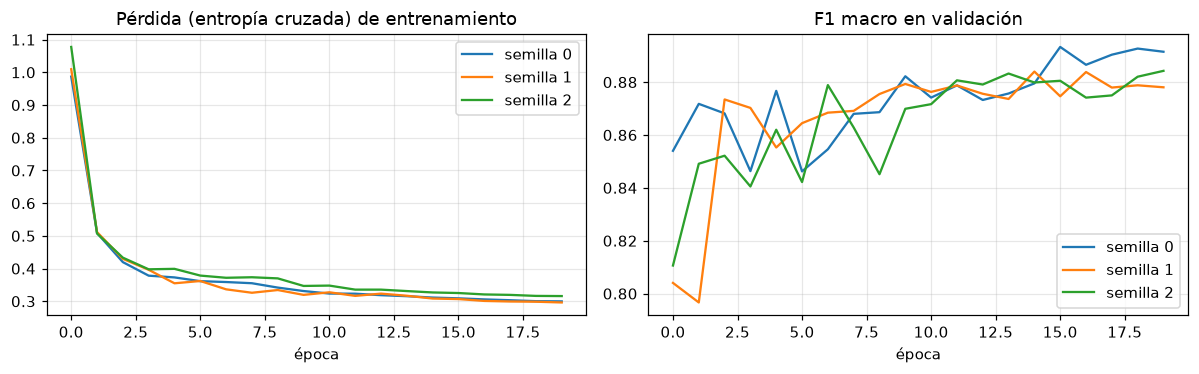
\includegraphics[width=\textwidth]{figures/curvas.png}
\caption{Entrenamiento de las tres semillas: pérdida (izquierda) y F1 macro en validación
(derecha).}
\end{figure}

\begin{table}[H]
\centering\small
\caption{Reporte por clase del QNN (semilla 0) en el conjunto de prueba.}
\begin{tabular}{lrrrr}
\toprule
Clase & Precisión & Exhaustividad & F1 & Soporte \\ \midrule
Barbunya & 0.856 & 0.657 & 0.744 & 397 \\
Bombay   & 0.994 & 0.987 & 0.990 & 156 \\
Cali     & 0.794 & 0.883 & 0.836 & 489 \\
Dermason & 0.908 & 0.913 & 0.910 & 1064 \\
Horoz    & 0.953 & 0.943 & 0.948 & 558 \\
Seker    & 0.942 & 0.934 & 0.938 & 608 \\
Sira     & 0.829 & 0.874 & 0.851 & 791 \\ \midrule
Macro    & 0.896 & 0.884 & 0.888 & 4063 \\
\bottomrule
\end{tabular}
\end{table}

\subsection{Comparación con modelos clásicos}
\begin{table}[H]
\centering\small
\caption{Resultados en el conjunto de prueba (4\,063 granos). El QNN aparece como media de 3
semillas.}
\begin{tabular}{@{}llrcc@{}}
\toprule
Modelo & Entrada & Parámetros & Accuracy & F1 macro \\ \midrule
\textbf{QNN re-uploading $L=4$} & 4 PCA (4 qubits) & 65 & 0.884 & 0.886 \\
Centroides más cercanos & 4 PCA & -- & 0.804 & 0.810 \\
Regresión logística & 4 PCA & 35 & 0.887 & 0.890 \\
MLP 6 neuronas & 4 PCA & 79 & 0.885 & 0.887 \\
Random Forest & 4 PCA & -- & 0.889 & 0.894 \\
MLP 64--32 & 4 PCA & 2\,631 & 0.890 & 0.894 \\
SVM RBF & 4 PCA & -- & 0.895 & 0.898 \\ \midrule
Random Forest & 16 caract. & -- & 0.919 & 0.931 \\
SVM RBF & 16 caract. & -- & 0.924 & 0.936 \\
MLP 64--32 & 16 caract. & 3\,399 & 0.926 & 0.937 \\
\bottomrule
\end{tabular}
\end{table}

\begin{figure}[H]
\centering
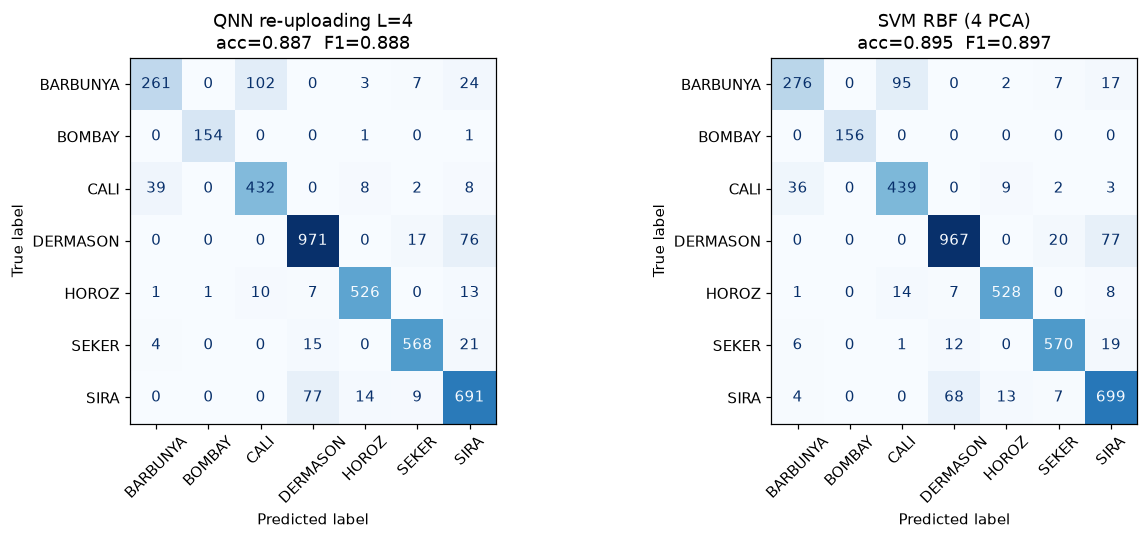
\includegraphics[width=\textwidth]{figures/conf_comp.png}
\caption{Matrices de confusión del QNN y del SVM-RBF (ambos con 4 componentes PCA). Los errores se
concentran en los mismos pares de clases.}
\end{figure}

\subsection{Ablaciones}
\label{sec:abl}
\begin{table}[H]
\centering\small
\caption{Ablación de arquitectura (semilla 0, prueba).}
\begin{tabular}{lcccc}
\toprule
Configuración & Parámetros & Accuracy & F1 macro \\ \midrule
$L=1$, re-subida & 17 & 0.611 & 0.455 \\
$L=2$, re-subida & 33 & 0.863 & 0.858 \\
$L=4$, re-subida (principal) & 65 & 0.887 & 0.888 \\
$L=6$, re-subida & 97 & 0.886 & 0.888 \\
$L=4$, \textbf{sin} re-subida (VQC) & 53 & 0.870 & 0.861 \\
\bottomrule
\end{tabular}
\end{table}

\begin{figure}[H]
\centering
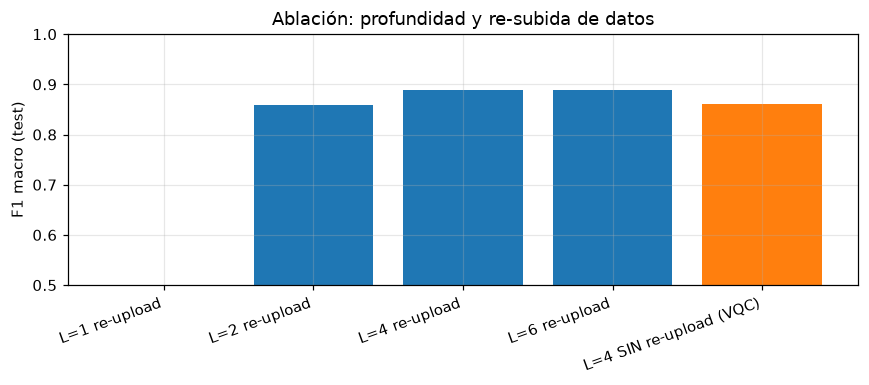
\includegraphics[width=.62\textwidth]{figures/ablacion.png}
\caption{F1 macro en prueba para distintas profundidades y con/sin re-subida de datos.}
\end{figure}

\subsection{Efecto del número de \emph{shots} y costo}
\label{sec:costo}
\begin{figure}[H]
\centering
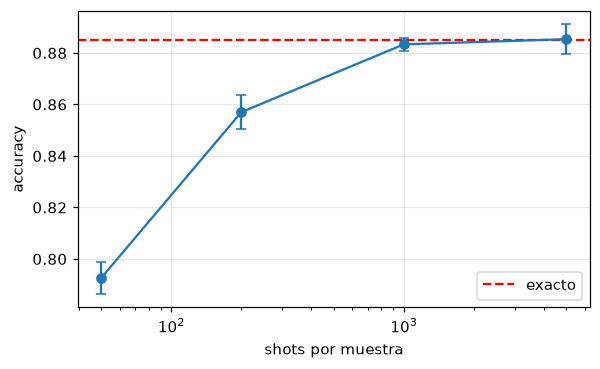
\includegraphics[width=.55\textwidth]{figures/shots.png}
\caption{\emph{Accuracy} del QNN entrenado al estimar $p_k$ con $S$ \emph{shots}. La línea roja
es la evaluación exacta ($0.885$ en esta submuestra).}
\end{figure}
Con 50, 200, 1\,000 y 5\,000 \emph{shots} la \emph{accuracy} es $0.793$, $0.857$, $0.883$ y $0.885$
respectivamente. El error estándar de una probabilidad estimada es $\sqrt{p(1-p)/S}$, por lo que
resolver diferencias entre clases cercanas exige $S=O(1/\varepsilon^2)$.

Para \emph{entrenar} en hardware con \emph{parameter-shift} y $S=1000$ se necesitarían
$8532\cdot2\cdot65\cdot1000\approx1.1\times10^{9}$ \emph{shots} por época y
$\approx2.2\times10^{10}$ en 20 épocas, frente a un único \emph{backward pass} clásico; la
inferencia sobre 4\,063 granos cuesta $\approx4\times10^{6}$ \emph{shots}.

%=====================================================================
\section{Discusión y conclusiones}
%=====================================================================
\begin{enumerate}[leftmargin=*]
\item \textbf{Competitividad.} Con 4 qubits y 65 parámetros, el QNN queda a $\approx1$ punto
porcentual de F1 del mejor modelo clásico con la misma entrada (SVM-RBF) y empata con un MLP de
capacidad comparable (79 parámetros). Con 4\,063 muestras de prueba el error estándar de una
\emph{accuracy} cercana a $0.89$ es $\approx0.5\%$, por lo que la diferencia es marginal. Supera
claramente al clasificador de centroides ($0.810$), lo que indica que la capacidad no lineal del
circuito aporta.
\item \textbf{El cuello de botella es la entrada.} Todos los modelos con 4 componentes se estancan en
$\approx0.89$--$0.90$; con las 16 características los clásicos llegan a $0.93$--$0.94$ de F1. Comprimir
a 4 componentes pierde información discriminante. Es una restricción \emph{cuántica} real: codificación
por ángulos implica un qubit por característica.
\item \textbf{Errores estructurales.} QNN y SVM confunden los mismos pares: Barbunya$\leftrightarrow$Cali
y Dermason$\leftrightarrow$Sira, que se solapan en el espacio PCA; Bombay es casi perfecta
(F1 $\approx0.99$). Barbunya, minoritaria, tiene la menor exhaustividad ($0.66$).
\item \textbf{La re-subida importa.} Con $L=1$ el modelo es insuficiente; a partir de $L=4$ se
satura. Sin re-subida (mismo $L$) el F1 baja $\approx2.7$ puntos, consistente con la teoría de
Fourier. Es una sola semilla: la magnitud es indicativa.
\item \textbf{Costo práctico.} En simulación el QNN tarda $\approx150$--$220$\,s por entrenamiento
frente a $0.3$--$10$\,s de los clásicos; en hardware, el entrenamiento y la inferencia requieren
muchas mediciones y el rendimiento depende del presupuesto de \emph{shots}.
\item \textbf{Ventaja cuántica: no.} En este problema un modelo clásico de 79 parámetros iguala al QNN
y modelos con más información lo superan, entrenando mucho más rápido. Un espacio de Hilbert de
dimensión 16 se simula trivialmente. El aporte es demostrar que un clasificador variacional compacto
y poco profundo (profundidad nativa 36, 16 CNOT) resuelve un problema multiclase real con un
rendimiento competitivo y caracterizar sus costos.
\end{enumerate}

\subsection*{Limitaciones y trabajo futuro}
Una sola partición train/test y tres semillas (una validación cruzada estratificada daría
intervalos de confianza más sólidos); hiperparámetros del QNN no optimizados exhaustivamente; sin
modelo de ruido de compuertas; no se implementó la variante de centroides cuánticos con
\emph{swap-test}. Como extensiones: más componentes PCA/qubits, lecturas con observables
$\langle Z_i\rangle$, simulación con ruido (Qiskit Aer) y mitigación de errores.

%=====================================================================
\section{Reproducibilidad}
%=====================================================================
El cuaderno \texttt{Proyecto\_Final\_Semillas\_QML.ipynb} se ejecuta completo (aprox.\ 25 minutos en
CPU) con el kernel \texttt{Python (compu\_cuantica)}. Todas las fuentes de aleatoriedad están
fijadas (partición con \texttt{random\_state=42}; semillas 0, 1 y 2 para el QNN; semilla del
muestreo de \emph{shots}). Si no encuentra \texttt{data/}, el cuaderno descarga el dataset de UCI.

%=====================================================================
\begin{thebibliography}{9}
\bibitem{koklu2020} M.\ Koklu e I.\ A.\ Özkan. \emph{Multiclass classification of dry beans using
computer vision and machine learning techniques}. Computers and Electronics in Agriculture,
174:105507, 2020. Dataset UCI \emph{Dry Bean}, DOI 10.24432/C50S4B.
\bibitem{perez2020} A.\ Pérez-Salinas, A.\ Cervera-Lierta, E.\ Gil-Fuster y J.\ I.\ Latorre.
\emph{Data re-uploading for a universal quantum classifier}. Quantum, 4:226, 2020.
\bibitem{schuld2021} M.\ Schuld, R.\ Sweke y J.\ J.\ Meyer. \emph{Effect of data encoding on the
expressive power of variational quantum-machine-learning models}. Phys.\ Rev.\ A, 103:032430, 2021.
\bibitem{havlicek2019} V.\ Havlíček et al. \emph{Supervised learning with quantum-enhanced feature
spaces}. Nature, 567:209--212, 2019.
\bibitem{mcclean2018} J.\ R.\ McClean et al. \emph{Barren plateaus in quantum neural network
landscapes}. Nature Communications, 9:4812, 2018.
\bibitem{bergholm2018} V.\ Bergholm et al. \emph{PennyLane: Automatic differentiation of hybrid
quantum-classical computations}. arXiv:1811.04968, 2018.
\bibitem{schuld2020} M.\ Schuld, A.\ Bocharov, K.\ M.\ Svore y N.\ Wiebe. \emph{Circuit-centric
quantum classifiers}. Phys.\ Rev.\ A, 101:032308, 2020.
\end{thebibliography}

\end{document}
